\documentclass[12pt]{article}
\usepackage{url}
\usepackage{utopia}
\usepackage[pdftex]{graphicx}

\begin{document}

\title{\textsc{Cheops} v1.0\\User Manual}
\author{Tristan Miller\\ \url{psychonaut@nothingisreal.com}\\ \url{http://www.nothingisreal.com/cheops/}}
\maketitle
\tableofcontents
\pagebreak

\section{Introduction}

This paper describes \textsc{Cheops} (\textsc{Ch}ess \textsc{o}pponent
\textsc{s}imulator), an object-oriented chess-playing program.

\section{Compiling \textsc{Cheops}}

A standard Makefile is provided; under most Unix systems simply typing
\texttt{make} will suffice.  For other systems, simply compile all the
\texttt{.cpp} files and link in the C++ math and standard template
libraries.  Use your compiler's optimization switch if desired.  Here
is an example which works with the GNU C++ Compiler:

\begin{quote}
\texttt{g++ -O3 -o cheops.exe cheops.cpp ChessBoard.cpp StdAfx.cpp Player.cpp HumanPlayer.cpp ComputerPlayer.cpp move.cpp -lstd++ -lm}
\end{quote}

\section{Running \textsc{Cheops}}

Due to the limitations of its Spartan user interface, it is
recommended that \textsc{Cheops} be run in a text mode supporting at
least fifty lines. In MS-DOS, this may be accomplished by typing
\texttt{mode con lines=50}. If launching the program from a Windows
95/98 shortcut, activate the shortcut properties window and select an
appropriate screen size from \emph{Initial size} drop-down list box
under the \emph{Screen} tab.

\begin{figure}[htbp]
  \begin{center}
    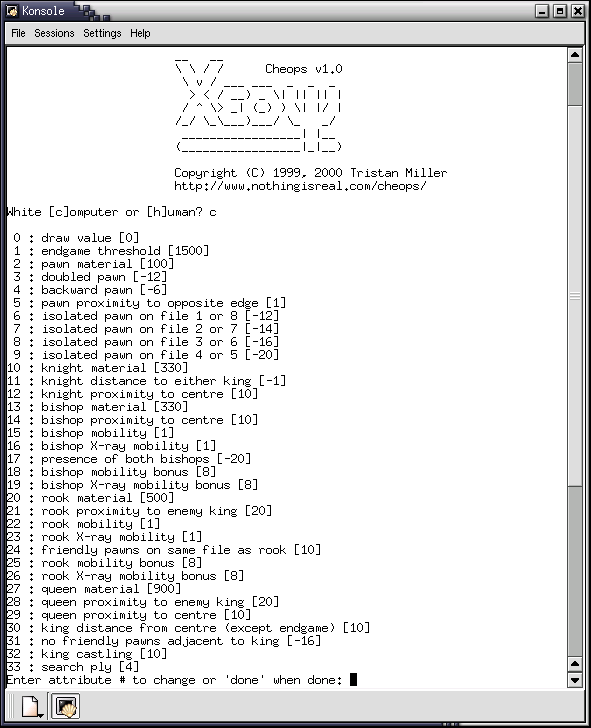
\includegraphics[width=6cm]{cheops1.png}
    \caption{Setting the static evaluation function weights}
    \label{fig:weights}
  \end{center}
\end{figure}

To start the program, simply type \texttt{cheops} at the command line.
There are no command-line parameters. Once \textsc{Cheops} is invoked,
the program displays a title screen and prompts the user for who
controls each player. If a computer opponent is chosen, a list of
default static evaluation function weights is displayed. (See Figure
\ref{fig:weights}.)  To accept the default values, type \texttt{done};
otherwise, enter the number of the weight to change. The program will
then prompt for the new value. The program will allow the user to
adjust the weights until \texttt{done} is entered.

\begin{figure}[t]
  \begin{center}
    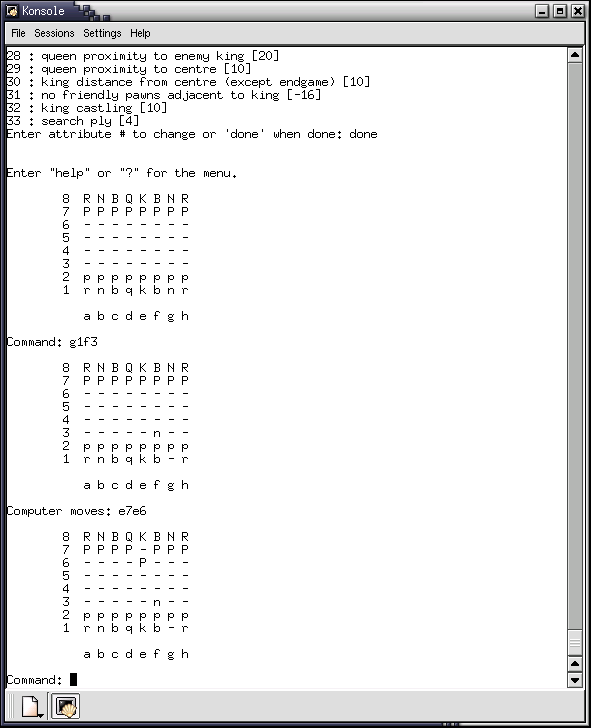
\includegraphics[width=6cm]{cheops2.png}
    \caption{Moving pieces}
    \label{fig:move}
  \end{center}
\end{figure}


Following player setup, the board is displayed and the game begins.
The board is represented by a simple ASCII diagram using the standard
one-character piece abbreviations; white pieces are represented by
small letters and black pieces by capitals.  Each player makes his
move in turn; human players are prompted for their move, and computer
players move automatically. To make a move, enter the source and
destination coordinates in standard algebraic notation---for example,
\texttt{g1f3} moves the knight at g1 to f3.  (See Figure
\ref{fig:move}.) For pawn promotions, the promotion piece must be
appended---for instance, \texttt{e7e8n} promotes to a knight. For
castling, the user may either enter the source and destination
coordinates of the king, or he may simply type \texttt{o-o} or
\texttt{o-o-o} for kingside or queenside castling, respectively. The
players may continue entering moves in this manner until a checkmate
or draw state is reached. As in regular chess, a draw occurs upon
stalemate, triple observance of the same board configuration with the
same side to move, or observance of fifty moves without a capture or
pawn advance.

In addition to legal moves, the following commands are also available
as responses for human players. At the end of a game, no further moves
are possible, and one of these commands must be entered.

\begin{description}
\item[resign] forfeits the match
\item[bd] redisplays the board
\item[coords] toggles display of board coordinates
\item[reverse] reverses board display (black on top to white on top, or vice versa)
\item[think] toggles display of computer ``thinking''
\item[log] display log of moves for the current game
\item[save] saves the move log to a file
\item[new] starts a new game (board in initial configuration with white to move)
\item[who] set players and computer stats, if applicable
\item[quit] exits the program
\end{description}

\section{Development}

\subsection{Program structure}

\textsc{Cheops} is comprised of four classes and a main program which
provides an interface and ties everything together. The
\texttt{ChessBoard} class is at the heart of the program; it is a
fully encapsulated data structure allowing for the manipulation of
chessboards and the pieces thereon contained. The board itself is
represented by a privately-declared 64-element array, each cell
containing an enum value representing the type and colour of the
piece.\footnote{In the early stages of design, the idea of defining a
  separate class for each piece type, complete with movement rules,
  was contemplated.  Following admonisitns from other C++/Java
  programmers who had followed this route and found it to
  unnecessarily complicate and slow their code \cite{smaaland}, this
  approach was decided against.} There are also numerous flags and
counters, the purposes of which should be obvious from the source code
and its internal documentation. The class has just two major public
functions---\texttt{can{\textunderscore}move()}, which returns a
boolean value indicating whether or not a given move is valid; and
\texttt{do{\textunderscore}move()}, which actually performs a move,
rearranging the pieces on the board and updating the appropriate
status flags. In addition to these, there are a score of small inline
functions for performing menial status checks and type conversions.
These functions add an extra layer of abstraction within the class,
permitting the implementation of the board and pieces to be changed
without having to modify the other functions in the class or its
friends. Even the board arithmetic is self-contained to a
degree---individual squares are represented not by integers 0 to 63
but by enum constants \texttt{a1} to \texttt{h8}, and incrementing
ranks and files is done using constants \texttt{Rank} and
\texttt{File}. This data hiding would make it easy to change the board
array to, say, the popular 10 $\times$ 12 or 0x88 formats
\cite{eppstein}.

The remaining three classes define the players. At the top of the
hierarchy is \texttt{Player}, an abstract base class serving as a
template for its two derived classes, \texttt{HumanPlayer} and
\texttt{ComputerPlayer}.  The \texttt{Player} class itself is very
small and contains no executable functions. It has just three main
members: one boolean flag indicating whether the player is human, and
two pure virtual functions, the first of which is used to get commands
from the player, and the second to modify his\footnote{Read ``his'' as
  ``his or her'' for the entirety of this document.} stats. In
\texttt{HumanPlayer}, the first function prints out the familiar
command prompt and relays the input back to the main program, while in
\texttt{ComputerPlayer} it runs the minimax search algorithm to come
up with the optimal move.  The second function, while vestigial in
\texttt{HumanPlayer}, is used in the other class to set the weights
for the static evaluation function.

The \texttt{ComputerPlayer} class is one of the largest in
\textsc{Cheops}, and thus deserves particular notice here. Because it
needs to examine in detail the state of the chessboard,
\texttt{ComputerPlayer} is a friend class of \texttt{ChessBoard}. It
includes functions for determining potential moves, finding the
distance between two board squares, assessing board configurations,
and, of course, choosing the optimal move using a minimax search of
the game tree. The actual criteria used to evaluate a particular board
position are many and varied, and are treated specifically in the
following section.

\subsection{Static evaluation function}

The heuristics for the positional evaluator of \textsc{Cheops} are
based on those of \textsc{GNU Chess} \cite{stanback} and \textsc{Cray
  Blitz} \cite{crayblitz}. Many of the criteria involve a calculation
of distance between squares on the board; this distance function
varies with the type of piece under consideration.  For example,
queens can move along any line, while rooks can move only on ranks and
files; thus, the span between two fixed squares is not always
equidistant for queens and rooks. Using the standard (Euclidean) means
of computing distance is not feasible, even as an approximation, as it
uses relatively slow floating-point calculations.  Thus, functions
were derived for actual piece-wise distance, which were later found to
have been previously discovered and named by mathematicians
\cite{wilson}.  ``Rook-wise'' distance is known in mathematics as
Manhattan distance, and is represented by the following general
formula: \[ D(x, y) = \sum_{i=1}^{m} \left|x_i - y_i\right|. \]
``Queen-wise'' distance, known as Chebychev distance, is given by the
following function: \[ D(x, y) = \max_{i=1}^{m} \left|x_i -
  y_i\right|. \] Kings, which move the same as queens, also use
Chebychev distance. Except that they can only reach half the squares
on a chessboard, bishops also measure distance Chebychev-style. For
knights and their unusual L-shaped moves, no suitable distance
function could be found, so either of the above-noted functions is
used as an approximation in the program.

Following is a detailed description of the static evaluator; any
numerical constants cited refer to default values which may be changed
by the user.

The base material value of a pawn is 100 points. Isolated pawns (those
which have no friendly pawns on adjacent files) are given a penalty
which is a function of the file they occupy: pawns on the outermost
files lose 12 points, those on files 2 and 7 lose 14, those on 3 and 6
lose 16, and those on the innermost lose 20. Pawns whose advance is
restrained by an opposing pawn on an adjacent file, and which have no
friendly pawn to support that advance, are considered to be backward,
and lose 6 points. Doubled pawns---that is, pawns which occupy a file
containing other friendly pawns---are penalized 12 points. Finally,
pawns are given a bonus for proximity to the opposite edge of the
board, effectively receiving 1 point for each square distant from
their home edge.

Knights start off at 330 points, and are given a 1-point penalty for
each square distant from either king. Knights are also given a bonus
for inverse Chebychev distance to the centre; the bonus starts at 0 in
the corners and increases by a factor of 10 per square towards the
centre.

Bishops also have a base value of 330 points. The presence of both
king's and queen's bishops is necessary to avoid a penalty of 20
points. Individual bishops receive bonuses for proximity to centre,
calculated and weighted (by default) in the same manner as for
knights. Bishops also receive a bonus for mobility and X-ray mobility
through pieces except pawns. This bonus is 1 point for every square
under attack, plus a one-time 8-point bonus for attacks on an enemy
queen, rook, or king. The weights for the mobility and X-ray mobility
attacks are separately adjustable.

A rook is worth 500 points initially. Rooks receive a bonus for
inverse Manhattan distance to the enemy king; the bonus increases by
20 points for every square closer to the king. Mobility and X-ray
mobility bonuses are handled the same as those for bishops, and while
the default weights are the same, they are independently adjustable.
Also, rooks lose 10 points for the presence of friendly pawns on their
file.

Queen heuristics are very simple: they start off at 900 points and
receive bonuses for their proximity to the centre (in increments of
10) and to the enemy king (in increments of 20).

A king has no material value; such a number would be irrelevant as the
capture of the king signals the end of the game. Instead, kings are
given a penalty in steps of 10 for their proximity to the centre of
the board. This penalty is a function of the stage of the game, which
is determined by the combined base material value of the remaining
pieces. If this sum is below a user-defined threshold (default 1500),
the board is considered to be in endgame and the centre penalty is
lifted. Kings are given a 20-point bonus for castling, and a 16-point
penalty if they occupy a square which has no immediately adjacent
friendly pawns.

The score for a board is, in effect, the sum of the scores of the
opponent's pieces subtracted from the sum of the scores of the current
player's pieces. If the static evaluator inspects a board in
checkmate, however, this evaluation algorithm is dispensed with and
the board is given a score of positive or negative infinity, depending
on which side has been mated. For obvious reasons, this score is not
user-adjustable. For a draw, however, the board value is user-defined
(default 0). The rationale for this decision is for chess matches:
when a computer has won the first four games in a six-game match, for
example, there is no further need to win subsequent games; a draw may
therefore be valued as a win ($+\infty$). On the other hand, a
computer losing 2--3 should count a draw as a loss ($-\infty$) in the
sixth and final game.


\subsection{Game tree search}

\textsc{Cheops} uses as its game tree search a standard minimax search
with alpha--beta cutoff. One feature which was planned but dropped
from the implementation was the option to time-limit the computer
opponent's moves. It was felt that this option was more trouble than
was worth to implement as it would have necessitated the installation
of an iterative deepening algorithm. Such a feature would have
resulted in better gameplay at the cost of exponentially longer
thinking time. The human playtesters found that using a regular three-
or four-ply search, typically completed within ten seconds, was
challenging enough for them.

Another feature left out of the final release was the option for
players (human or computer) to offer draws. It was decided that having
the computer offer a draw would be a sure sign to its opponent that it
is losing. Conversely, a computer opponent should never accept a draw
offer, even if it is losing, since the possibility should always be
reserved for the human making a mistake should the game continue. That
said, heuristics for forced draws (stalemates, triple occurrence, and
the fifty-move rule) were still included in the program; a winning
program will generally avoid such a condition.

\subsection{User interface}

\textsc{Cheops} features only a simple ASCII board display and
command-line interface reminiscent of GNU Chess \cite{gnuchess}.
Rather than have the static evaluation function weights read from a
file, as originally planned, a menu-based system was implemented
allowing the user to conveniently view and change individual weights
as the program is running. For reasons of portability, \textsc{Cheops}
assumes nothing about the user's display terminal, and as such, long
streams of output are not paused after every page. Experience has
shown that the program is best run in an environment which supports at
least fifty rows and forty columns, and/or in a windowing system that
includes a scroll-back buffer.  Because of the highly modularized
nature of the \textsc{Cheops} source code, it would not be difficult
to add a system-dependent GUI for input and output.

\section{Licence}

This manual and the software it accompanies \copyright 1999, 2000
Tristan Miller.  \textsc{Cheops} is Free Software. It can be freely
used, modified, and distributed under the terms of the GNU General
Public Licence.  You should have received a copy of the GNU General
Public Licence along with this program in the file LICENCE; if not,
write to the Free Software Foundation, Inc., 59 Temple Place---Suite
330, Boston, MA 02111--1307, USA.

\begin{thebibliography}{99}

\bibitem{eppstein} Eppstein, D. ``Board representations.''
  \emph{Game Programming}.
  \url{http://www.ics.uci.edu/~eppstein/180a/s97.html}  (14 April 1997)

\bibitem{gnuchess} \emph{GNU Chess 4.0.pl77}.  Free Software
  Foundation.  \url{ftp://prep.ai.mit.edu/pub/gnu/gnuchess/} (10 May 1999)

\bibitem{crayblitz} Hyatt, R.~M., A.~E.~Gower and H.~L.~Nelson.
  ``Cray Blitz.'' \emph{Computers, Chess, and Cognition}.  New York:
  Springer--Verlag, 1989.

\bibitem{smaaland} Smaaland, G.  \emph{Computer Chess
    Programming}.  \url{http://www.mi.uib.no/~gautes/cchess.html}
  (1 July 1999)

\bibitem{stanback} Stanback, J.  ``Heuristic descriptions for
  \emph{CHESS}.''  \emph{GNU Chess}.  Free Software Foundation, 1987.
  \url{http://www.imsa.edu/~stendahl/comp/txt/gnuchess.txt} (11 May 1999)

\bibitem{wilson} Wilson, D.~R.~and T.~R.~Martinez. ``Improved
  heterogeneous distance functions.''  \emph{Journal of Artificial
    Intelligence Research}, 6 (1997) pp.~1--34

\end{thebibliography}

\end{document}
